%! Author = Tom
%! Date = 07.12.2022
\section{Einleitung}

In diesem Kapitel wird an das Thema und die Motivation dieser Arbeit herangeführt.
Außerdem wird definiert, welche Ziele diese Arbeit erreichen soll und eine grobe Übersicht über die
Kapitelstruktur gegeben.

\subsection{Motivation}

Mit einer steigenden Nutzung von GraphQL wird es immer wichtiger, geeignete Tests für GraphQL-API's zu entwickeln damit eine
gute Softwarequalität sichergestellt werden kann. Idealerweise können diese Testtools solche API's automatisch testen,
so wie es für REST-API's schon umgesetzt wurde. Die Struktur von GraphQL erlaubt allerdings zyklische Strukturen
und ermöglicht somit ein potentenziell undendlich großen Testraum.
In einem Paper "Automatic Property-based Testing of GraphQL-API's" (hier Quelle) wurde versucht ein solches
automatisches Testtool schon umzusetzen. Allerdings hat dieses Paper zwei große Verbesserungspunkte. 
Einerseits die Art, wie die Tests generiert werden, andererseits die Auswertung der Tests.

\subsubsection*{Testgenerierung}

Bei der Testgenerierung wurde mit den zyklischen Strukturen in GraphQL Schemas so
umgegangen, dass eine Rekursionstiefe definiert wurde, damit man das Problem des unendlichen Testraumes beheben kann.
Dieser Ansatz erlaubt es aber leider nicht, dass eine ideale Abdeckung (was das ist wird später genau
definiert) gewährleistet werden kann.
Insbesondere komplexere, zyklische Strukturen werden hierbei von dem automatischen
Tool nicht getestet da die Rekursionstiefe dies oft nicht erlaubt.
Mit der Nutzung von graphspezifischen Algorithmen ist es jedoch möglich Graphabdeckungen zu ermitteln auch wenn diese
eine zyklische Struktur haben und somit kann algoritmisch das Problem des Papers gelöst werden.
In dieser Arbeit sollen diese graphspezifischen Algorithmen implementiert werden und dann mittels Datengeneratoren eigenständig
Tests erzeugen.

\subsubsection*{Testauswertung}

Die Auswertung der Tests ist im Paper darauf basierend, dass die zu testende API vor allem auch funktionale Korrektheit überprüft wird,
dies bedeutet insbesondere, dass hier die HTTP-Status Codes von Anfragen ausgewertet werden sowie GraphQL eigene Statusmeldungen untersucht werden.
Ein richtiger Abgleich im Test findet nicht statt, es wird lediglich überprüft ob der Rückgabe-Datentyp dem erwarteten Datentyp entspricht.
Es wäre jedoch besser wenn nicht nur der Rückgabe-Datentyp stimmt sondern auch der Inhalt in diesem Datentyp. In dieser Arbeit
soll das Programm mittels eines Orakels verbessert werden. Dies bedeutet, dass die GraphQL API mit Testdaten befüllt wird und Anfragen
gestellt werden können, die sich dann auch logisch ineinander auflösen. Hierbei ist insbesondere zu beachten, dass Kreisstrukturen sich in gewisser Weise
in sich selbst auflösen, d.h. Eingabeobjekt = Ausgabeobjekt.

\subsection{Umsetzung}

Zuallererst wird in dieser Arbeit etwas Theorie definiert und in Bezug gesetzt. Angefangen mit einer allgemeinen Definition
eines Graphens im mathematischen Sinne und GraphQL als Schnittstelle, wird dann ein Bezug dieser beiden Themen
zueinander hergestellt. Wenn der Bezug von Graphentheorie und GraphQL klar ist, wird der eigentliche Algorithmus für die
ideale Abdeckung des Graphens algorithmisch erklärt, eine Anwendung auf GraphQL in der Theorie gezeigt und bewiesen.
Danach werden die theoretischen Erkenntnisse in einem praktischen Projekt umgesetzt. Hierbei wird ein Tool erstellt,
welches aufgrundlage des Überdeckungsalgorithmus & einem Datengenerator Tests erstellt und dann auswertet mittels
den alten bzw. erweiterten Ablgeichsmethoden. Um zu zeigen, dass das neue Verfahren eine Verbesserung darstellt wird dann
ein Benchmark Test zwischen altem und neuen System erstellt. Bei diesem Benchmark Test werden 3 verschiedene
GraphQL-Schemas getestet, 2 Schemas aus dem alten Paper, hier ergibt sich ein direkter Vergleich an z.B. generierten Tests und
Graphabdeckung. Im 3ten Schema wird ein speziell sehr zyklisches Schema ausgewertet um zu zeigen, dass einerseits die Implementierung
den Algorithmus korrekt umsetzt und wie groß die Verbesserung in solchen Schemas dann sind.










































\begin{description}
    \item[Positionierung neuer Produkte]
    \item[Optimale Verteilung von Produkten für kurze Wege]
    \item[Effiziente Bestandshaltung von Produkten]
\end{description}


\begin{figure}[!htbp]
    \begin{center}
        \begin{tikzpicture}[-,>=stealth',shorten >=1pt,auto,node distance=2cm,
        thick,main node/.style={circle,draw,font=\Large\bfseries}]
        \node[main node] (1) {1};
        \node[main node] (2) [below left of=1] {2};
        \node[main node] (3) [below right of=1] {3};
        \node[main node] (4) [below of=2] {4};
        \node[main node] (5) [below of=3] {5};

        \draw (1) to (2);
        \draw (1) to (3);
        \draw (2) to (4);
        \draw (3) to (5);
        \draw (4) to (5);
        \draw (1) to [bend right] (3);
        \draw (2) to (5);

        \end{tikzpicture}
        \caption{Ein Graph}
        \label{fig:simple-graph}
    \end{center}
\end{figure}


\subsection{Graphen}

Ein Graph ist definiert als eine Menge von Knoten N und Kanten E

\subsection{GraphQL}

GraphQL ist eine Art, Schnittstellen zu definieren. Insbesondere die Kommunikationsart/Anfrageart an diese Schnittstelle
wird in dieser Art mithilfe von Graphen umgesetzt. Hierzu existiert ein Schema, welches die Struktur der Daten in einen
Graphen formatiert.

\subsection{Testen von Software}

Damit Software zuverlässig läuft muss die getestet werden.

\subsection{Kritik am Paper und Ausblick für die Arbeit}



Um eine höhere Komplexität abbilden zu kennen wird das Graphenmodell um eine Typisierung erweitert.
Typsierte Graphen bestehen aus zwei Teilen. Einerseits dem Typgraphen, dieser stellt einen Bauplan für den tatsächlichen
genutzen Graphen dar und dem Instanz-Graphen, welcher dann den konkreten Graphen darstellt.
Ein typisierter Graph ist ein spezifischer Graph, der eine Typisierung der einzelnen Knoten vorsieht.
Abbildung 1.1 zeigt eine beispielhafte Lösung für unser Problem. Der exakte Typgraph wird aber später näher definiert wenn
die Anforderungen an die Software erhoben wurden und man somit eine konkretere Vorstellung der Modellierung.

\begin{figure}[!htbp]
    \begin{center}
        \begin{tikzpicture}
            \node (1)[abstract, rectangle split, rectangle split parts=2] at (4, 8)
            {
                \textbf{Lagersystem}
                \nodepart{second} Properties
            };
            \node (2)[abstract, rectangle split, rectangle split parts=2] at (4, 6)
                {
                \textbf{Lager}
                \nodepart{second} Properties
            };
            \node (3)[abstract, rectangle split, rectangle split parts=2] at (4, 4)
                {
                \textbf{Regal}
                \nodepart{second} Properties
            };
            \node (4)[abstract, rectangle split, rectangle split parts=2] at (4, 2)
                {
                \textbf{Lagerplatz}
                \nodepart{second} Properties
            };
            \node (5)[abstract, rectangle split, rectangle split parts=2] at (2, 0) % geteilter Platz
                {
                \textbf{Sammelprodukt}
                \nodepart{second} Properties
            };
            \node (6)[abstract, rectangle split, rectangle split parts=2] at (8, 0)
                {
                \textbf{Einzelprodukt}
                \nodepart{second} Properties
            };

            \draw (1) edge node { unterhält } (2) ;
            \draw (2) edge node [loop right] { Entfernung zueinander } (2);
            \draw (3) edge node [loop right] { Entfernung zueinander } (3);
            \draw (2) edge node { besitzt } (3);
            \draw (3) edge node { bietet Platz } (4);
            \draw (4) edge node { beinhaltet } (5);
            \draw (4) edge node { beinhaltet } (6);
        \end{tikzpicture}
    \caption{Ein beispielhafter Typgraph}
    \label{fig:wt2}
    \end{center}
\end{figure}

und in Abbildung 1.3 sein Instanzgraph der nach dem Bauplan vom Typgraphen erstellt wurde.
Ein Knoten der Klasse Lagersystem ist somit die Wurzel des Graphens. Das Lagersystem hat dann 1..n Lager. Jedes dieser Lager
hat dann Regale welche die Laufwege und Entfernungen zu den anderen Regalen als Kanten haben. Außerdem hat jedes Regal
Kanten zu Lagerplätzen, dies sind die Lagerplätze innerhalb des Regals. Jeder Lagerplatz beeinhaltet dann entweder ein
Einzelprodukt oder ein Sammelprodukt.

\begin{figure}[!htbp]
    \begin{center}
        \makebox[\textwidth]{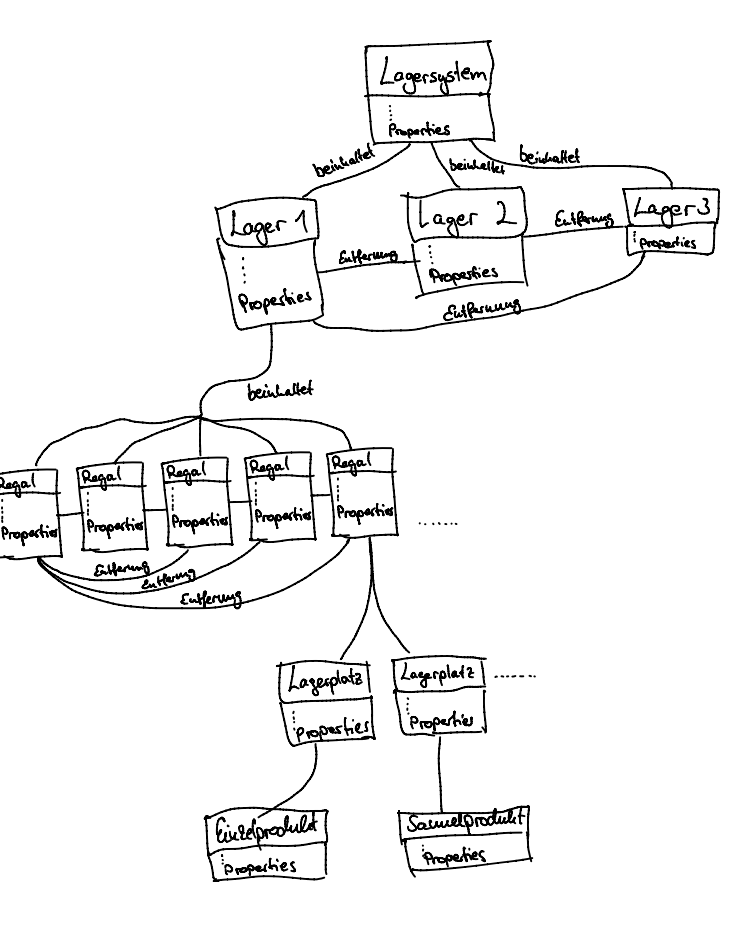
\includegraphics[width=\paperwidth]{../images/instance-graph}}
        \caption{Instanzgraph}
    \end{center}
    \label{fig:figure}
\end{figure}

Ziel der Arbeit soll nun sein, ein System zu entwickeln in dem solche Typgraphen gebildet werden können und dann, nach
individueller Konfiguration, optimiert werden.
Hierbei soll vor allem auf die Optimierung hinsichtlich unser Eingangs genannten Ziele geachtet werden:
\begin{description}
    \item[Positionierung neuer Produkte]
    \item[Optimale Verteilung von Produkten für kurze Wege]
    \item[Effiziente Bestandshaltung von Produkten]
\end{description}

\section{Technische Umsetzung}
Die Nutzung der Graphoptimierungen wird stark mit Drittsystemen zusammenarbeiten. Heutzutage fast jedes Lager eine
WMS-Software in der Nutzung welche die Geschäftsprozesse eines Lagers abbildet. In einigen dieser Systeme sind einige Optimierungen
schon eingebaut, jedoch nicht in dem großen Umfang und der Modellierungsfeinheit wie hier. Da jedoch eine komplette Umstellung
einerseits logistisch riesige Aufwände nach sich ziehen würde sowie den Rahmen dieser Arbeit sprengen würde, soll das Optimierungssystem
ein eigenständiges System sein welches seine Verbesserungen an das WMS dann meldet.




















